\documentclass{article}
\usepackage{amssymb,amsfonts,amsmath,amsthm,latexsym}
\usepackage{subfigure}
\usepackage{float}
\usepackage{graphicx}
\usepackage{booktabs}
%\usepackage{fontspec,xltxtra,xunicode}
%\usepackage{times}

%----------
% 定义中文环境
%----------

\usepackage{xeCJK}
\usepackage[pdfborder={0 0 1},colorlinks,linkcolor=red,anchorcolor=blue,citecolor=green]{hyperref}

\setCJKmainfont[BoldFont={SimHei},ItalicFont={KaiTi}]{SimSun}
\setCJKsansfont{SimHei}
\setCJKfamilyfont{zhsong}{SimSun}
\setCJKfamilyfont{zhhei}{SimHei}
\setCJKfamilyfont{zhkai}{KaiTi}
\setCJKfamilyfont{zhfs}{FangSong}
\setCJKfamilyfont{zhli}{LiSu}
\setCJKfamilyfont{zhyou}{YouYuan}

\newcommand*{\songti}{\CJKfamily{zhsong}} % 宋体
\newcommand*{\heiti}{\CJKfamily{zhhei}}   % 黑体
\newcommand*{\kaiti}{\CJKfamily{zhkai}}  % 楷体
\newcommand*{\fangsong}{\CJKfamily{zhfs}} % 仿宋
\newcommand*{\lishu}{\CJKfamily{zhli}}    % 隶书
\newcommand*{\yuanti}{\CJKfamily{zhyou}} % 圆体

%----------
% 版面设置
%----------
%首段缩进
\usepackage{indentfirst}
\setlength{\parindent}{2em}

%行距
\renewcommand{\baselinestretch}{1.4} % 1.4倍行距

%页边距
\usepackage[a4paper]{geometry}
\geometry{verbose,
  tmargin=2cm,% 上边距
  bmargin=2cm,% 下边距
  lmargin=3cm,% 左边距
  rmargin=3cm % 右边距
}


%----------
% 其他宏包
%----------
%图形相关
\usepackage[x11names]{xcolor} % must before tikz,x11names defines RoyalBlue3
\usepackage{graphicx}
\usepackage{pstricks,pst-plot,pst-eps}
\usepackage{subfig}
\def\pgfsysdriver{pgfsys-dvipdfmx.def} % put before tikz
\usepackage{tikz}

%原文照排
\usepackage{verbatim}

%网址
\usepackage{url}



%==========
% 正文部分
%==========

\begin{document}

\title{基于卷积神经网络的图像分类系统}
\author{李逸岩, 黄喆敏, 林子宏}
%\date{} % 若不需要自动插入日期,则去掉前面的注释;{ } 中也可以自定义日期格式
\maketitle

\section{任务介绍}
CIFAR-10 数据集由60000张图片组成,每张图片的大小为32 $\times$ 32,RGB三通道。整个数据集都被标记为十个标签的一种。数据集在下载后已经被分为5个训练Batch和1个测试Batch。每个Batch都包含10000张图片。\cite{2009learning}

\subsection{工作概述}
此Project进行CIFAR-10数据集的图像分类,需要基于CNN。由于数据集已经进行打包,我们直接使用数据集的训练集-测试集分类方法。我们完成的工作包括数据预处理,设计模型,设计训练策略,实际训练,进行训练总结(以文字和可视化的形式)。我们的模型主要采用PyTorch进行训练,基于\url{https://pytorch.org/tutorials/beginner/blitz/cifar10_tutorial.html},以及ResNet模型。 \\
\indent
在没有使用额外数据以及预训练模型的前提下,我们设计的模型\textbf{准确率最高达到了92\%, 参数大小为83MB}。 此外,按照要求,随机数种子被设为2021,便于审阅我们的结果; 如果想复现我们的结果,请参阅README.md。

\subsection {相关研究}
对于图像识别问题,主流模型包括Transformer\cite{dosovitskiy2021image},ResNet\cite{kolesnikov2020big},EfficientNet\cite{tan2021efficientnetv2},DCN\cite{sousa2021cnn},ResNeXt\cite{Li_2019_CVPR}等。\\

\indent 2015年何恺明等人提出的ResNet模型\cite{resnet2016}是图像识别领域的一个里程碑,它引入了残差模块,解决了CNN中深度网络难以训练的问题;近年来,\textbf{Transformer}模型开始崭露头角。传统意义上,Transformer领域主要用来解决自然语言处理的相关任务。然而,最近一些文章开创性地\textbf{将Transformer模型跨领域地引用到了计算机视觉中}。这些文章所提出的模型用self-attention机制替代CNN中的卷积操作,并且取得了很好的效果。\cite{dosovitskiy2021image}

\indent 对于此Project使用的CIFAR-10数据集,在\\
\url{https://paperswithcode.com/sota/image-classification-on-cifar-10} 中含有使用此数据集模型排名。从2012年有记录以来,SOTA模型的准确率从88.8\%提高到了99.5\%。发表于CVPR2021的ViT-H/14将准确率提高到了99.5\%\cite{dosovitskiy2021image},而使用CNN的FlexConv在达到92.2\%以上准确率的同时\cite{romero2021flexconv},保证了自己的参数大小约为0.67MB,约为准确率最高的模型的$\frac{1}{1000}$。


\section{数据处理}
我们采取了以下数据预处理方式:
\begin{itemize}
\item 随机裁剪(Random Crop)
\item 随机水平翻转(Random Horizontal Flip)
\item 随机仿射变换(Random Affine)
\item 颜色抖动(Color Jitter)
\end{itemize}

\begin{figure}[H]
	\centering
	\subfigure[原始数据集]{
		\centering
		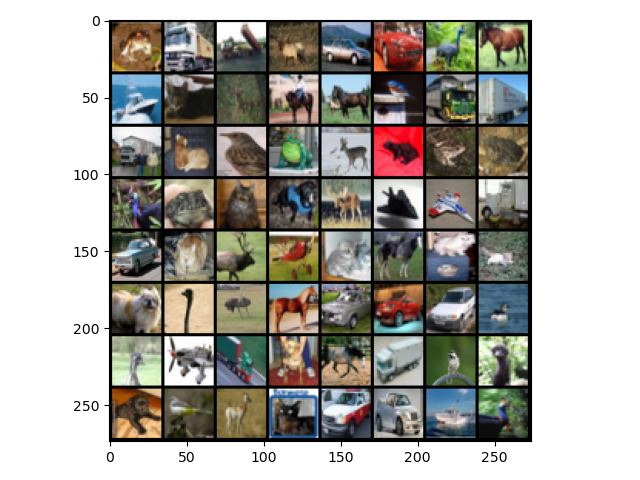
\includegraphics[width=0.4\linewidth]{original_dataset}
	}
	\subfigure[扩充数据集1]{
		\centering
		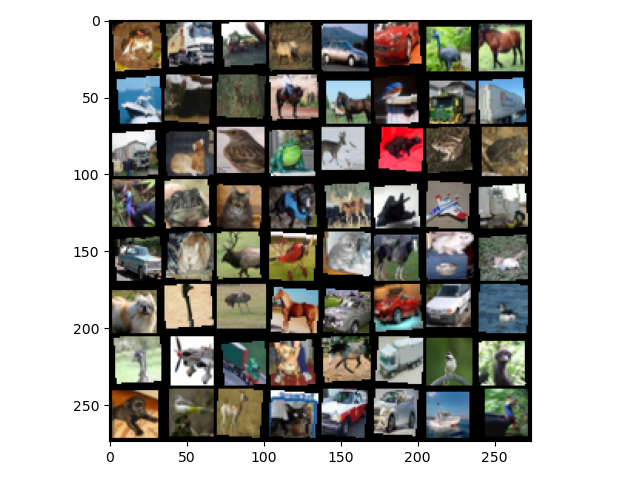
\includegraphics[width=0.4\linewidth]{augment1}
	}
	\subfigure[扩充数据集2]{
		\centering
		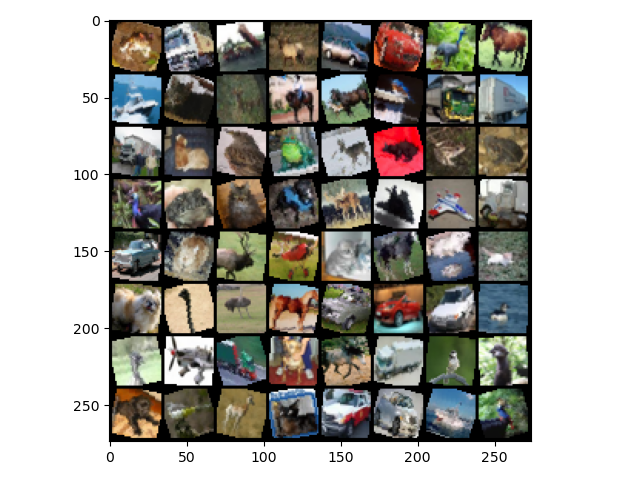
\includegraphics[width=0.4\linewidth]{augment2}
	}
	\subfigure[扩充数据集3]{
		\centering
		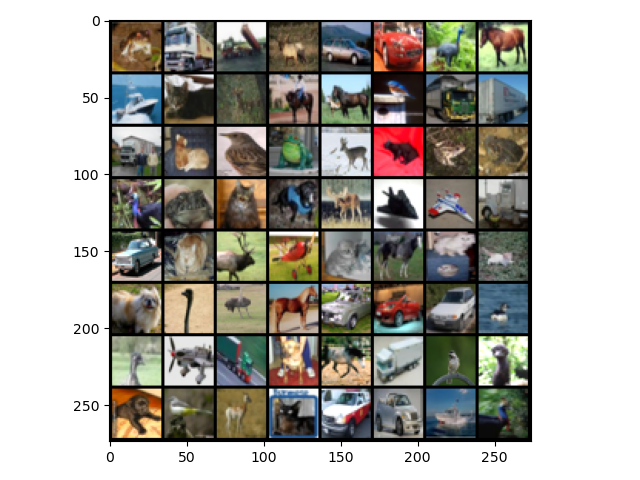
\includegraphics[width=0.4\linewidth]{augment3}
	}
	\caption{原始数据集,扩充数据集1(随机裁剪+随机水平翻转+随机仿射变换),扩充数据集2(随机放射变换),扩充数据集3(颜色抖动)。}
\end{figure}
通过图像增强,我们扩充了数据集,为训练提供了更多样本。数据增强的效果,对比与可能有效的原因您可以在5.3.4查看。

\section{系统设计}
\subsection{架构选择}
\subsubsection{ResNet}
由于此Project的要求为\textbf{模型需要基于CNN},因此我们采用了ResNet作为主要模型。

ResNet是时下应用最广泛的基于CNN的图像分类模型。\cite{he2015deep} 该模型的提出让CNN的层数由原来的不到十层提高到了上百层甚至上千层。
原先人们发现随着CNN层数的增多,模型准确度反而下降。而这不能用过拟合来解释(因为训练集和测试集的Loss都同步上升),而随着BN算法(Batch Normalization)在很大程度上解决了梯度消失/爆炸问题后\cite{batch},模型退化问题仍然存在。这表明这可能是CNN架构本身的问题带来的。
\\ 
\indent
为了解决这个问题,\textbf{ResNet提出了Shortcut方法},引入了恒等映射,让模型拥有了“什么都不做”的选择,有效防止了更多的层数带来的信息丢失。而更多的层数为分层学习提供了可能,每一层学到更细化的特征,提高了模型的表达能力;从而提高了模型的准确度。\cite{resnet2016}
\\ 
\indent
我们在研究ResNet的机制时,特别注意到了\textbf{ResNet没有引入Dropout机制}。Dropout是一种常见的正则化技术,可以有效缓解过拟合。\cite{dropout2014}但是在许多流行的网络,例如ResNet\cite{he2015deep}、ResNeXt\cite{xie2017aggregated}中,都没有采用Dropout。
一些研究发现,Dropout在网络测试时神经元会产生\textbf{方差偏移}(variance shift),这会导致当Dropout与Batch Normalization同时被使用时,效果反而更差。\cite{li2019understanding}因此,我们采取了单独使用BN算法的方法。
\\ 
\indent
我们的模型是基于ResNet的基本框架,进行调参。在ResNet论文\cite{he2015deep}中提出了5种ResNet模型,即ResNet-18,ResNet-34,ResNet-50,ResNet-101,ResNet-152. 数字代表的是层数,我们尝试复现了以下框架。\ref{Fig.resnet1}
%% 一张
\begin{figure}[h] %H为当前位置,!htb为忽略美学标准,htbp为浮动图形
	\centering %图片居中
	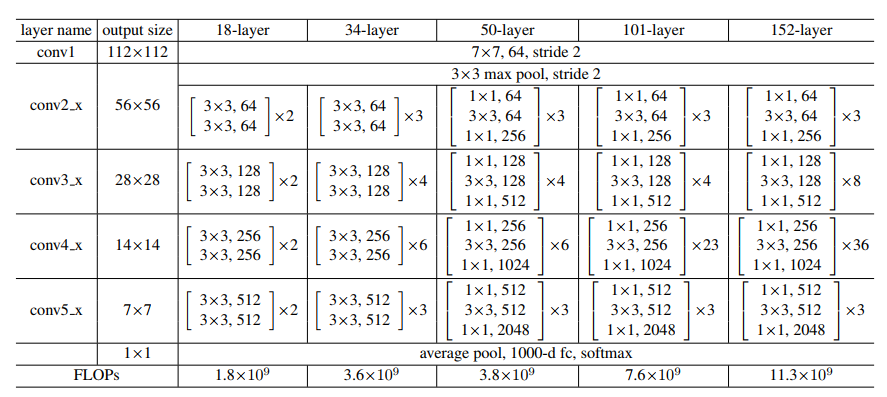
\includegraphics[width=0.85\textwidth]{resnet.png} %插入图片,[]中设置图片大小,{}中是图片文件名
	\caption{ResNet 论文中给出的模型结构} %最终文档中希望显示的图片标题
	\label{Fig.resnet1} %用于文内引用的标签
\end{figure}
\\
\indent
但是,在层数升至50层以上时,即便使用多块RTX3080 Ti显卡进行训练,也需要数小时甚至十余小时才能完成训练。因此,我们优先将有限的资源使用在了低层数的ResNet上。特别对ResNet-18(便于调参与快速训练查看结果)以及ResNet-50(较好的平衡了层数和训练速度)进行了调参和训练。在最后,我们尝试进行了ResNet-101的训练,事实证明,ResNet让模型层数更高,准确度也变得更好。
\\
\indent

\subsubsection{其他模型选择}
除了ResNet,我们还研究并且使用典型参数运行了一些在ResNet出现之前的较浅的CNN模型,包括Vgg-16,Inception-10, AlexNet-8。 我们阅读了这些模型的TensorFlow实现并且试着本地运行了他们。您可以在Appendix A中审阅这些结果。我们发现无论如何调整epoch的大小,这些模型的训练结果都明显不如我们选择的ResNet。因此,我们没有对这些模型进行进一步的调参和设计。

\subsection{ResNet架构说明}
上面提到了ResNet为新增加的层数引入了恒等映射的可能。我们希望能对$F(x) = H(x) - x$进行学习,因此学习到的原始特征应为$F(x) + x$. 这样残差为0时就是恒等映射了。\\
\begin{figure}[h] %H为当前位置,!htb为忽略美学标准,htbp为浮动图形
	\centering %图片居中
	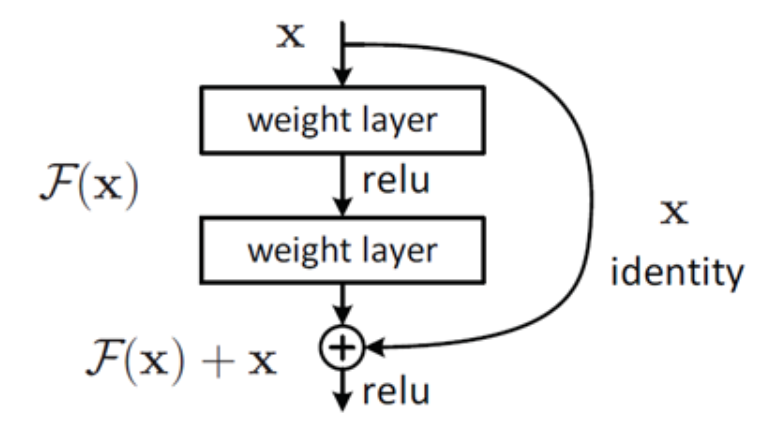
\includegraphics[width=0.5\textwidth]{resnetUnit.png} %插入图片,[]中设置图片大小,{}中是图片文件名
	\caption{ResNet 论文中的unit} %最终文档中希望显示的图片标题
	\label{Fig.resnet2} %用于文内引用的标签
\end{figure}
\indent
ResNet论文中提出了两种残差函数(Residual Function)。 一种应用于ResNet-18、ResNet-34较浅的网络,另一种应用于ResNet-50及更深的网络。 我们采用了这种模型设计。您可以在resnet\_all.py下面看到我们实现的两个残差单元~\ref{Fig.resnet4}。左图适用于层数较浅的网络,右图加入了\textbf{瓶颈层}(Bottle Neck Layer),可以减少参数的数量,适用于层数较深的网络。
此Project模型的主要架构由ResNet论文架构指导~\ref{Fig.resnet1},对残差单元~\ref{Fig.resnet4}进行组装得到的,在常见的数据集,例如CIFAR-10,ImageNet等,都有很好的表现。\\
\begin{figure}[h] %H为当前位置,!htb为忽略美学标准,htbp为浮动图形
	\centering %图片居中
	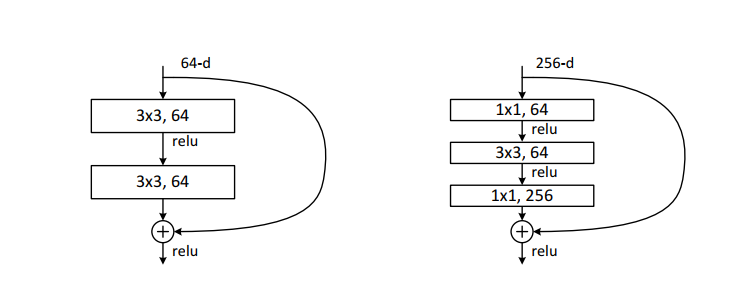
\includegraphics[width=0.95\textwidth]{resnet2units.png} %插入图片,[]中设置图片大小,{}中是图片文件名
	\caption{ResNet 论文中的两种unit,我们在代码中分别进行了实现} %最终文档中希望显示的图片标题
	\label{Fig.resnet4} %用于文内引用的标签
\end{figure}
\indent
此外,我们将超参数抽离为变量,将数据预处理,模型调用和结果展示记录抽取出来,放在train.py中方便进行训练,实验和展示。您可以在上述两个代码文件中审阅我们的模型和训练计划。下图是结合了残差单元和架构说明对ResNet-18的架构进行了更加清晰的展示。
\begin{figure}[h] %H为当前位置,!htb为忽略美学标准,htbp为浮动图形
	\centering %图片居中
	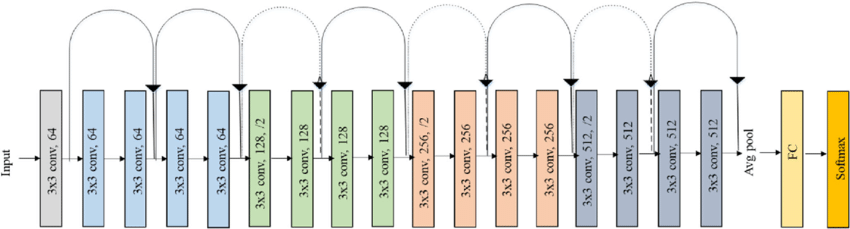
\includegraphics[width=0.95\textwidth]{resnet18.png} %插入图片,[]中设置图片大小,{}中是图片文件名
	\caption{ResNet-18 网络结构图} %最终文档中希望显示的图片标题
	\label{Fig.resnet3} %用于文内引用的标签
\end{figure}


\section{训练方法}
\subsection{超参数调试方法}
尽管我们尽可能提高了算力,但是限于ResNet的高层数, 我们的实验次数受到了限制,只能选择有限的超参数进行调试。ResNet论文\cite{he2015deep}为一些超参数提供了建议,比如Batch size为128, learning rate为0.1。基于此,使用ResNet-18架构,我们选择了以下参数进行调试:
\begin{itemize}
	\item Loss function: 损失函数指明了模型的训练目标, 我们对此进行了调研。
	\item Epochs: epoch过高可能导致过拟合,准确率下降。我们在一定的范围内选取epoch。
	\item Batch size: 我们调整Batch size至不同的数量级,直到占用的资源超过显存大小。
	\item Learning Rate: 我们从$8\times 10 ^ {-4}$开始,每隔一个量级,调整学习率大小。
	\item Learning Rate Decay: 我们选取PyTorch中几种学习率调整方法进行比较。
	\item Optimizer: 我们阅读论文,筛选出了SGD和Adam这两个优化器进行比较。\cite{keskar2017improving}同时调整优化器参数,包括weight decay 和momentum。
\end{itemize}

\subsection {Loss function}
尽管有人指出ResNet损失函数使用Binary Cross Entropy Loss的表现略好于Cross Entropy Loss\cite{beyer2020imagenet},但我们并没有把重点放在损失函数的选取上。我们选择了多分类问题最常使用的Cross Entropy Loss函数。

\subsection{Epoch}
在模型超参数调试完成之后,我们发现每次epoch在我们的训练集群上需要20秒左右训练。考虑到训练和实验的总规模,我们把epoch总数定为100和200两个milestore。 100 epochs达到时按要求记录报告准确率。为了挖掘模型的最大准确率,我们手动设置了200 epochs为最大的迭代次数,超过200 epochs自动停止。
当然,许多模型会运行300个甚至更多epochs,以提高准确度。\cite{xie2017aggregated}限于算力,我们只运行200个并且保存测试集上工作的最好的参数报告。

\subsection{Batch size}
我们从8开始,依次调整Batch size为8, 16, 64, 128, 256。其中,Batch size为256时,根据ResNet论文\cite{he2015deep} 建议,我们将learning rate设置为默认值的$110\%$,并且使用了2块GPU并行训练,满足显存要求。
由于显存限制,我们无法进一步提高Batch size,否则训练速度可能会迅速下降。实验完成后,我们选择最好的Batch size进行下一步调试。

\subsection{Learning rate}
我们从$1 \times 10^{-4}$开始,依次提高learning rate为$1 \times 10^{-3}$, $1 \times 10^{-2}$, $1 \times 10^{-1}$, 观察learning rate在哪个数量级表现最好,并且能平衡模型收敛所需要的时间。我们在这个数量级上进一步调试,直到选择一个比较好的learning rate进入下一步调参。

\subsection{Learning rate decay}
PyTorch中主要支持6种学习率调整方法。一般而言,训练初期给予较大的学习率,随着训练进行,学习率逐渐减小能较好的平衡训练速度和准确率。在我们阅读的论文中,常使用的decay方法为\textbf{StepLR}(等间隔调整学习率,调整倍数为$\gamma$倍,调整间隔为step\_size epochs)和 \textbf{CosineAnnealingLR}(以余弦函数为周期,在每个周期最大值时重新设置学习率)。
在一篇基于ResNet的论文中\cite{loshchilov2017sgdr},作者建议采用\textbf{warm restart}的方法调整学习率,并且在CIFAR-10数据集上进行了测试,效果较好。warm restart是指每隔若干步“重启”学习率,将学习率重新调整为初始学习率,然后再照常衰减。因此,CosineAnnealingLR较为合适。我们使用CosineAnnealingLR作为学习率衰减策略。

\subsection{Optimizer and weight decay}
常见的优化器包括SGD, Adam, LAMB。 大部分的卷积神经网络都采用了SGD作为优化器,也有人采用Adam作为优化器,而近几年的论文也有建议采用LAMB的。在近年的准确率最高的模型论文中,作者指出在ResNet-50模型中,各个优化器的表现是几乎没有差别的。\cite{dosovitskiy2021image}\\
\indent
根据一个深度学习科学家的回答\cite{QuoraAnswer},使用带动量的梯度下降法(SGD with momentum)更擅长于寻找"high-quality and flat"的局部最小值,而Adam则更容易找到"sharp"的局部最小值。前者带来了更好的泛化性和更低的性能损失,而且能够在其他超参数没有调试好的前提下带来还不错的结果。\\
\indent
我们同时尝试了SGD with momentum和 Adam, 其中前者的momentum 和weight\_decay 都采用了SGD优化器中的默认值,也即$momentum = 0.9, weight\_decay = 5 \times 10 ^ {-4}$;而Adam优化器的参数采纳了官方文档的推荐值,也即$lr = 1 \times 10^{-3}, \space betas=(0.9, 0.999), \space eps = 10 ^ {-8}, \space weight\_decay = 0$. (betas 为一阶和二阶的指数衰减率)我们对比了他们的效果,选择了相对更优秀的进行训练。

\section{实验与结果}
\subsection{平台}
由于ResNet对于GPU的要求较高,特别地,当Batch size较大时,会产生显存不够的情况。因此,我们使用了矩池云平台进行训练,租用了至多4块RTX3080 Ti显卡,CPU为8 $\times$ Xeon E5-2682 v4核心,86G内存,可同时训练至少4个模型。同时对于层数较多的模型,我们采取了2块GPU并行训练的方法。系统环境为Python3.7,CUDA 11.1,cuDNN 8.0.5,PyTorch 1.8.1,Horovod 0.22.1,Ubuntu 18.04。

\subsection{示例代码}
使用示例代码运行100 epochs查看结果作为baseline。

\subsection{超参数调试结果}
\subsubsection{Batch size}
在合理范围内,增大Batch size可以提高显存的利用率,矩阵乘法的并行效率提高,跑完一次epoch所需的迭代次数减少。但是,当Batch size过大时,显存容量可能不够,并且对参数的修正会更加缓慢。
因此,我们以ResNet-18为基准,按照8,32,64,128的顺序不断调整Batch size进行测试,得到图\ref{fig:resnet18_batchsize}所示的结果。
\begin{figure}[H]
	\centering
	\subfigure[训练集损失曲线]{
		\centering
		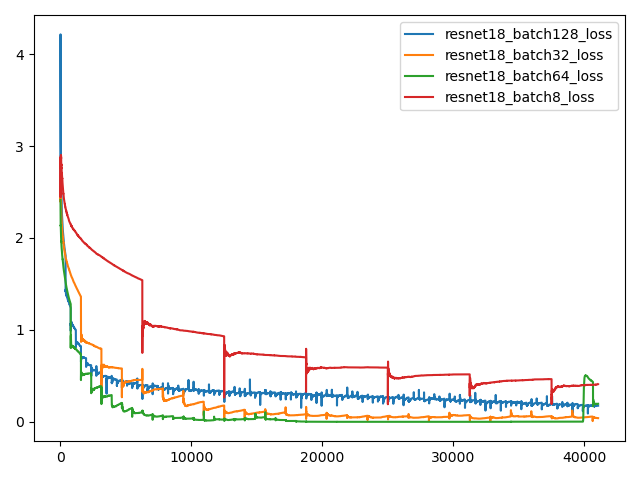
\includegraphics[width=0.45\linewidth]{train_loss_batchsize}
	}
	\subfigure[测试集准确率]{
		\centering
		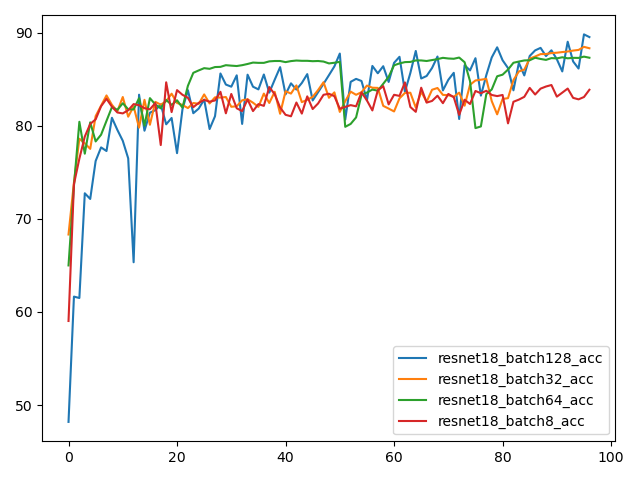
\includegraphics[width=0.45\linewidth]{test_acc_batchsize}
	}
	\caption{ResNet-18在不同Batch size下的表现。}
	\label{fig:resnet18_batchsize}
\end{figure}
当Batch size为128时,无论是训练集损失还是测试集准确率的变化都比较平稳。在训练速度较快的同时,也能更好地利用GPU资源。受限于硬件资源,我们没有尝试更大的Batch size。
\subsubsection{Learning rate}
基于上述结果,我们继续使用以128为Batch size的ResNet-18。依次以$8\times10^{-1}$,$8\times10^{-2}$,$8\times10^{-4}$进行训练,最终得到图\ref{fig:resnet18_lr}所示的结果。
\begin{figure}[H]
	\centering
	\subfigure[训练集损失曲线]{
		\centering
		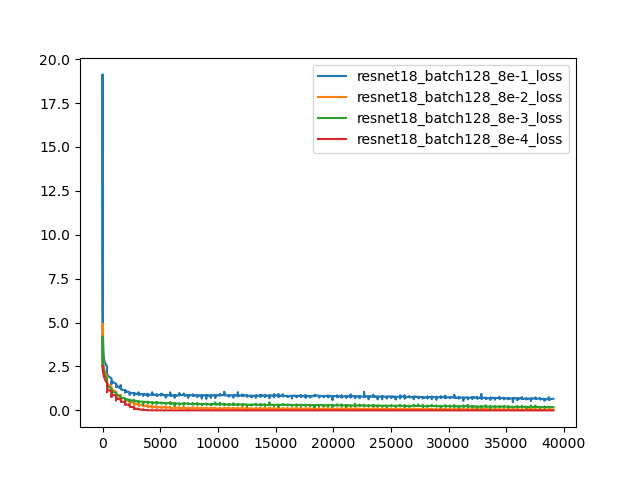
\includegraphics[width=0.45\linewidth]{train_loss_lr_1}
	}
	\subfigure[测试集准确率]{
		\centering
		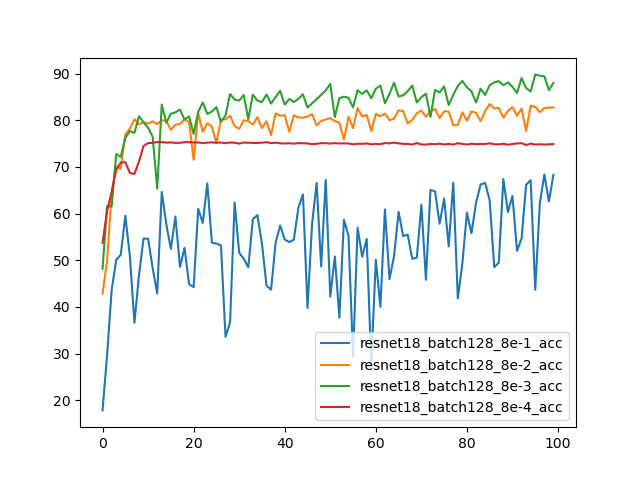
\includegraphics[width=0.45\linewidth]{test_acc_lr_1}
	}
	\caption{ResNet18在不同learning rate下的表现}
	\label{fig:resnet18_lr}
\end{figure}
结果表明过大的学习率可能导致准确率震荡的现象,而较小的学习率也可能会导致最终结果不够精确。对于ResNet-18而言,$8\times10^{-3}$和$8\times10^{-2}$都是较为合适的学习率——训练速度较快且训练过程波动小,较为稳定。最终我们选取$8\times10^{-3}$作为学习率。
\subsubsection{优化器}
在经过初步尝试后,我们发现
\subsubsection{预处理}
前文提到了我们使用的预处理方法。我们针对未扩充的原始数据集和扩充过的数据集进行了对照试验。图\ref{fig:resnet18_amp}展示了这一实验结果。
\begin{figure}[H]
	\centering
	\subfigure[训练集损失曲线]{
		\centering
		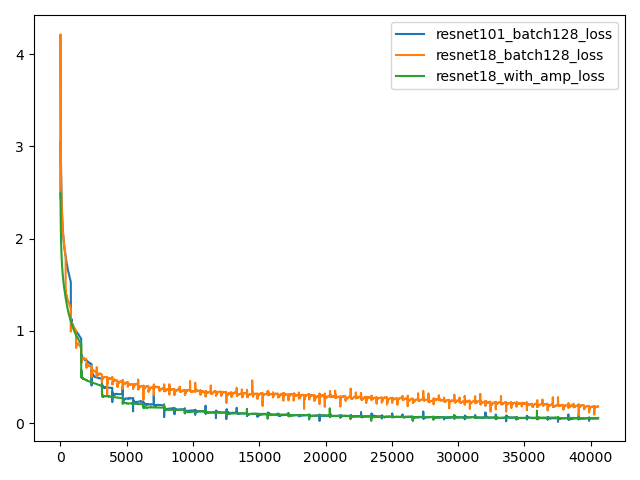
\includegraphics[width=0.45\linewidth]{train_loss_amp}
	}
	\subfigure[测试集准确率]{
		\centering
		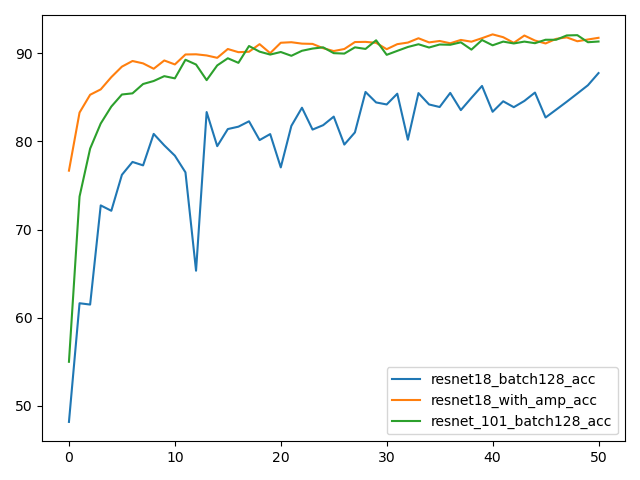
\includegraphics[width=0.45\linewidth]{test_acc_amp}
	}
	\caption{ResNet18使用原始数据集和扩充数据集的训练结果}
	\label{fig:resnet18_amp}
\end{figure}
扩充过的数据集的规模是原始数据集的四倍(包含原始数据集加上三个经过数据强化过的副本)。通过数据增强,我们获得了更多的数据样本。实验结果说明,这些数据样本提升了模型的准确率。随机翻转、随机仿射变换和颜色抖动等噪音使得模型学习到了更多特殊情况,增强了模型的泛化能力和鲁棒性。

与此同时,虽然样本数增多,但是ResNet自身的BN层等设计降低了过拟合发生的概率,最终得到了很高的测试集准确率。为了对比,我们还训练了ResNet-101,不难发现两者的最终结果相差的不多。通过预处理我们的模型预测能力获得了惊人的提升。

此外,我们发现,所有模型在训练集上的表现均显著优于测试集。以ResNet-18为例,在Batch size=64,且不加入数据增强的情况下,训练集的准确率可以达到100$\%$,但是测试集的准确率始终在85$\%$左右徘徊。这一现象的主要原因可能是测试集与训练集的分布差异(distribution gap); 另一部分原因可能是适应性差异(adaptivity gap), 即模型对于训练集产生了适应性的过拟合(adaptive overfitting)。\cite{cifar2018} 因此我们对训练集进行了数据增强,可以在一定程度上缓解这个问题。

\subsection{实验结果}
根据超参数调试结果,我们将基于准确率,训练时间,参数大小报告我们的实验结果。
\subsubsection{最终实验数据}
\begin{table}[h]
	\centering
	\caption{模型超参数}
	\begin{tabular}{l|l|l|l|l|l}
		\toprule
		Arch name & LR       & LR decay & Epochs   & Batch size & Warmup epochs \\ \midrule
		Res18     & 4.20E+07 & cosine   & 1.68E+06 & 1.06E+06   & 5             \\ \midrule
		Res50     & 8.55E+02 & cosine   & 3.42E+01 & 2.16E+01   & 5              \\ \midrule
		Res101    & 1.17E+03 & cosine   & 2.93E+04 & 4.64E+04   &  5            \\ \bottomrule
	\end{tabular}
\end{table}

\begin{table}[h]
	\centering
	\caption{模型优化器和损失函数}
	\begin{tabular}{l|l|l|l|l}
		\toprule
		Arch name & Optimizer& Weight decay & Dropout   & Loss           \\ \midrule
		Res18     & 4.20E+07 &         	    & No 	     & Cross Entropy  \\ \midrule
		Res50     & 8.55E+02 &              & No         & Cross Entropy  \\ \midrule
		Res101    & 1.17E+03 &              & No         & Cross Entropy  \\ \bottomrule
	\end{tabular}
\end{table}

\begin{table}[h]
	\centering
	\caption{模型运行环境和结果}
	\begin{tabular}{l|l|l|l|l}
		\toprule
		模型名称       & 运行时间      & 硬件         & 参数大小     & 准确率 	 \\ \midrule
		ResNet-18     & 4.20E+07     & 4.20E+07     & Cross Entropy  & 1897MB        \\ \midrule
		ResNet-50     & 8.55E+02     & 4.20E+07     & Cross Entropy  & LEVEL 8       \\ \midrule
		ResNet-101    & 1.17E+03     & 4.20E+07      & Cross Entropy &               \\ \bottomrule
	\end{tabular}
\end{table}



\subsection{训练过程}

我们对上述训练过程进行总结。所有模型的训练集误差均以较快的速度下降并在最终趋于平稳,但是准确率因模型的参数选定和结构而异。我们针对不同的参数进行了较多的测试,并将测试数据和LeNet进行比较,如图\ref{fig:total}所示。模型所用的参数如图例所示。其中,ResNet-50模型采用了2块GPU并行训练,其余均采用1块GPU训练。

\textbf{对于Batch size},我们分别尝试了Batch size=$8 / 32 / 64 / 128$的情况,此时learning\_rate$=8\times 10^{-3}$保持不变。

\textbf{对于learning rate},我们分别尝试了learning\_rate=$8\times 10^{-4} / 8\times10^{-3} / 8\times10^{-2} / 8\times10^{-1}$的情况,且保持Batch size=128不变。

\textbf{对于图像增强是否能提高训练速度/准确率},我们设计了两个模型进行比较。两个模型均为ResNet-18模型,Batch size=128,learning\_rate=$8\times10^(-3)$。其中一个模型的训练集使用了图像增强的训练集,另一个使用原始训练集。

其中,除了ResNet-18模型learning\_rate$=8\times 10^{-1}$时,\textbf{学习率较大导致无法收敛},所有的模型均好过LeNet。ResNet使得CNN网络可以非常深,以提取更深层次的特征,提升了准确率。但是一些未选定合适超参数的模型的表现可能还不如LeNet。这说明了选择合适参数的重要性。在深度学习领域,模型和参数是配套的,缺一不可。
\begin{figure}[H]
	\centering
	\subfigure[训练集损失曲线]{
		\centering
		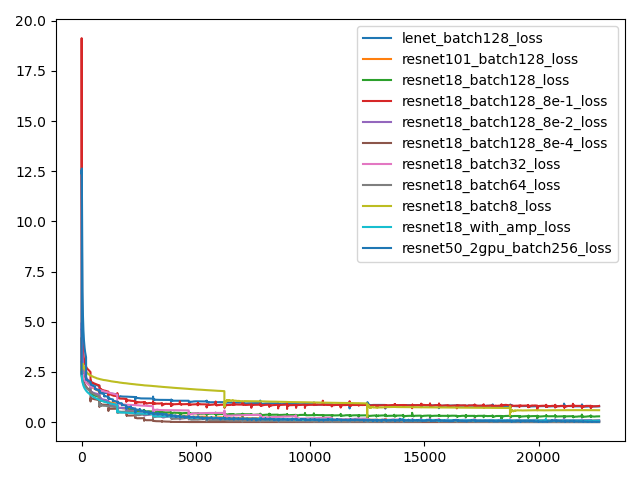
\includegraphics[width=0.46\linewidth]{total_train_loss}
	}
	\subfigure[测试集准确率]{
		\centering
		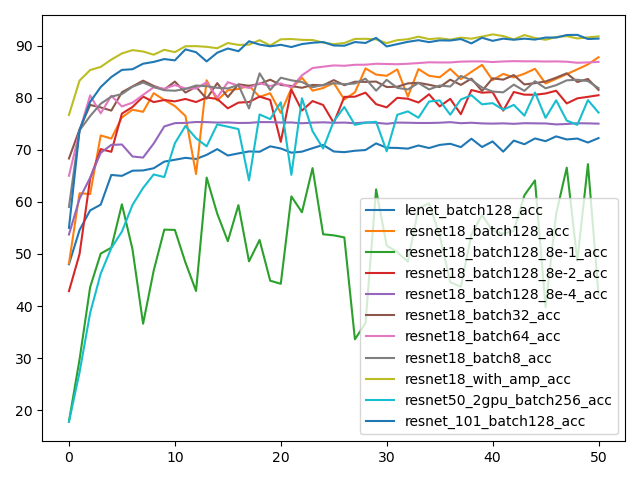
\includegraphics[width=0.46\linewidth]{total_test_acc}
	}
	\caption{实验测试结果汇总}
	\label{fig:total}
\end{figure}

% \subsubsection{图示训练过程}

\section{Appendix A}
在选择方向的过程中,我们回顾了自从CNN提出以来的各种模型以及其在数据集上的表现。对于这些模型,我们使用TensorFlow加以实现。您可以在./others里面查看这些模型并且复现结果。由于在部分模型中,数据对显存要求大于对显卡性能要求,我们没有保持硬件环境的严格一致,以求在花费尽可能低的情况下查看他们的效果。
\begin{table}[h]
	\centering
	\caption{各类模型的运行结果}
	\setlength{\tabcolsep}{0.6mm}{
		\begin{tabular}{l|l|l|l|l|l|l}
			\toprule
			Arch name   & Hardware            & Param size & Epochs & Batch size & Running time & Accuracy \\ \midrule
			VGG16       & Nvidia 3080 Ti       & 183.10 MB  & 100    & 32         & 61 mins      & 76.20\%  \\ \midrule
			alexnet8    & Nvidia Tesla T80    & 115.67 MB  & 100    & 32         & 145 mins     & 61.62\%  \\ \midrule
			resnet18-tf & Nvidia Tesla T4     & 134.16 MB  & 100    & 32         & 120 mins     & 73.07\%    \\ \midrule
			inception10 & Nvidia 3080 Ti       & 1.51 MB    & 100    & 32         & 59 mins      &  61.50\%    \\ \midrule
			lenet5 		& Nvidia 3080 Ti       & 0.24 MB    & 100    & 32         & 30 mins      &  56.87\%    \\ \bottomrule
		\end{tabular}
	}
\end{table}
\\
\indent
我们借此快速了解了各个模型的特点和能力,并且经过进一步了解,选择了ResNet继续研究。下图是这些模型的准确度,以及损失函数随迭代次数的变化示意图:
\begin{figure}[H]
	\centering
	\subfigure[AlexNet-8]{
		\centering
		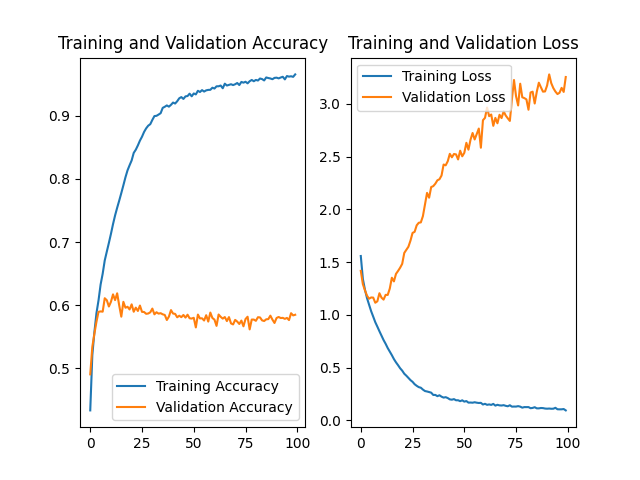
\includegraphics[width=0.4\linewidth]{alex8}
	}
	\subfigure[Vgg-16]{
		\centering
		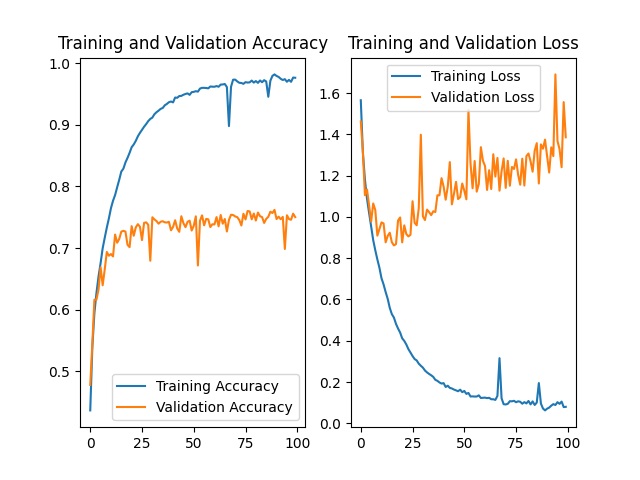
\includegraphics[width=0.4\linewidth]{vgg16}
	}
	\subfigure[Inception-10]{
		\centering
		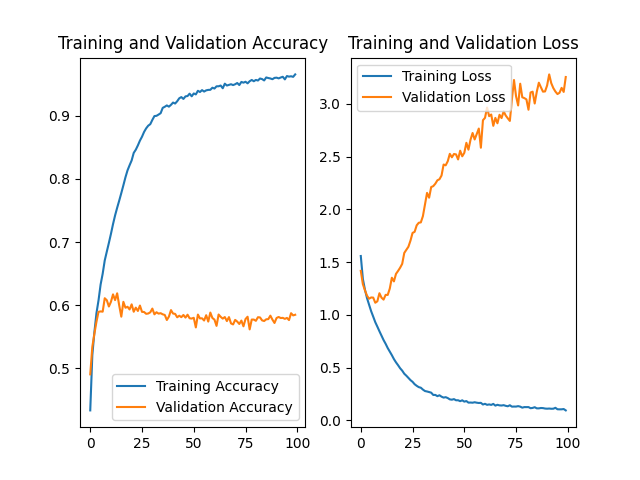
\includegraphics[width=0.4\linewidth]{inception10}
	}
	\subfigure[ResNet-18]{
		\centering
		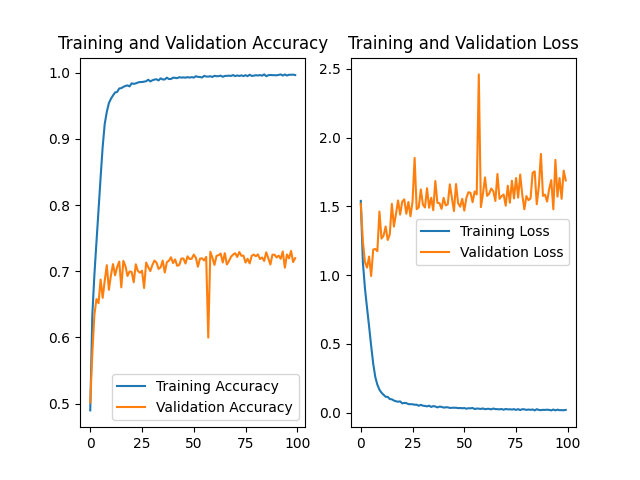
\includegraphics[width=0.4\linewidth]{resnet18-tf}
	}
	\subfigure[LeNet-5]{
	\centering
	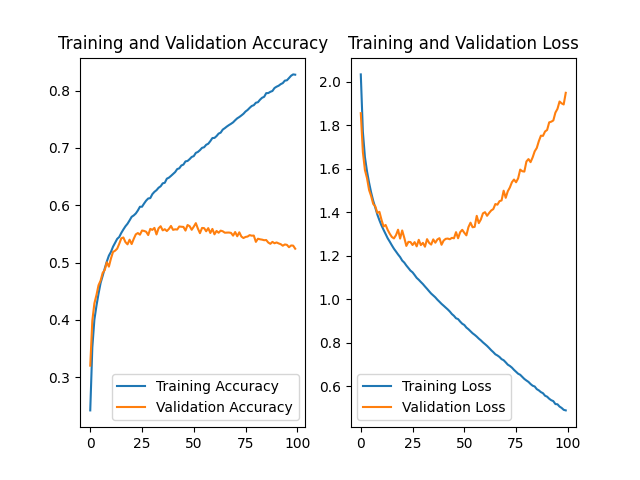
\includegraphics[width=0.4\linewidth]{lenet5}
}
	\caption{五种网络模型朴素实现的实验结果}
\end{figure}

\newpage
\nocite{*}
\bibliographystyle{ieeetr}
\bibliography{ref.bib}

\end{document}
